\chapter{Część implementacyjna}

\section{Zbiór narzędzi}
\begin{itemize}[leftmargin=1cm]
    \item Trello -- opracowanie zadań do poszczególnych etapów;
    \item Adobe XD -- prototypowanie aplikacji;
    \item Visual Studio Code -- środowisko programistyczne;
    \item Java 11 + Spring Boot -- backend;
    \item MongoDB -- baza danych;
    \item Angular 12 -- frontend;
    \item GitHub -- repozytorium kodu.
\end{itemize}

\section{Trello -- deklaracja zadań}
Pierwszy etap -> opracowanie zadań i funkcjonalności. Deklaracja tablic. Etapy implementacyjne -> 2 tyg czas trwania

\begin{figure}[H]
    \centering
    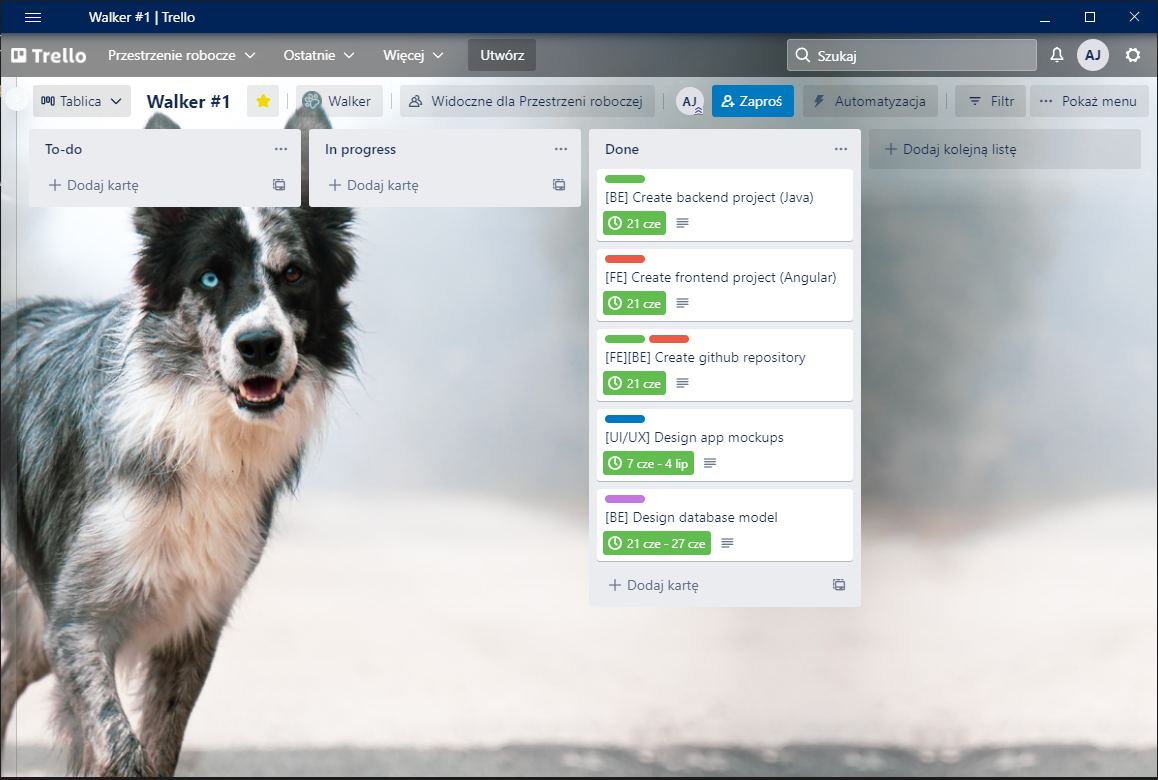
\includegraphics[width=0.7\linewidth]{rysunki/w1.PNG}
    \caption{Trello - tablica do pierwszego etapu}
    \label{fig:walker-board-1}
\end{figure}    

Opisy etykiet:
\begin{itemize}[leftmargin=1cm]
    \item Zielony -- zadania dotyczące backendu;
    \item Czerwony -- zadania dotyczące frontendu;
    \item Niebieski -- zadania dotyczące projektu UI/UX aplikacji;
    \item Fioletowy -- zadania dotyczące bazy danych
    \item Żółty -- zadania oznaczone jako bugi, problemy w programie
\end{itemize}

\begin{figure}[H]
    \centering
    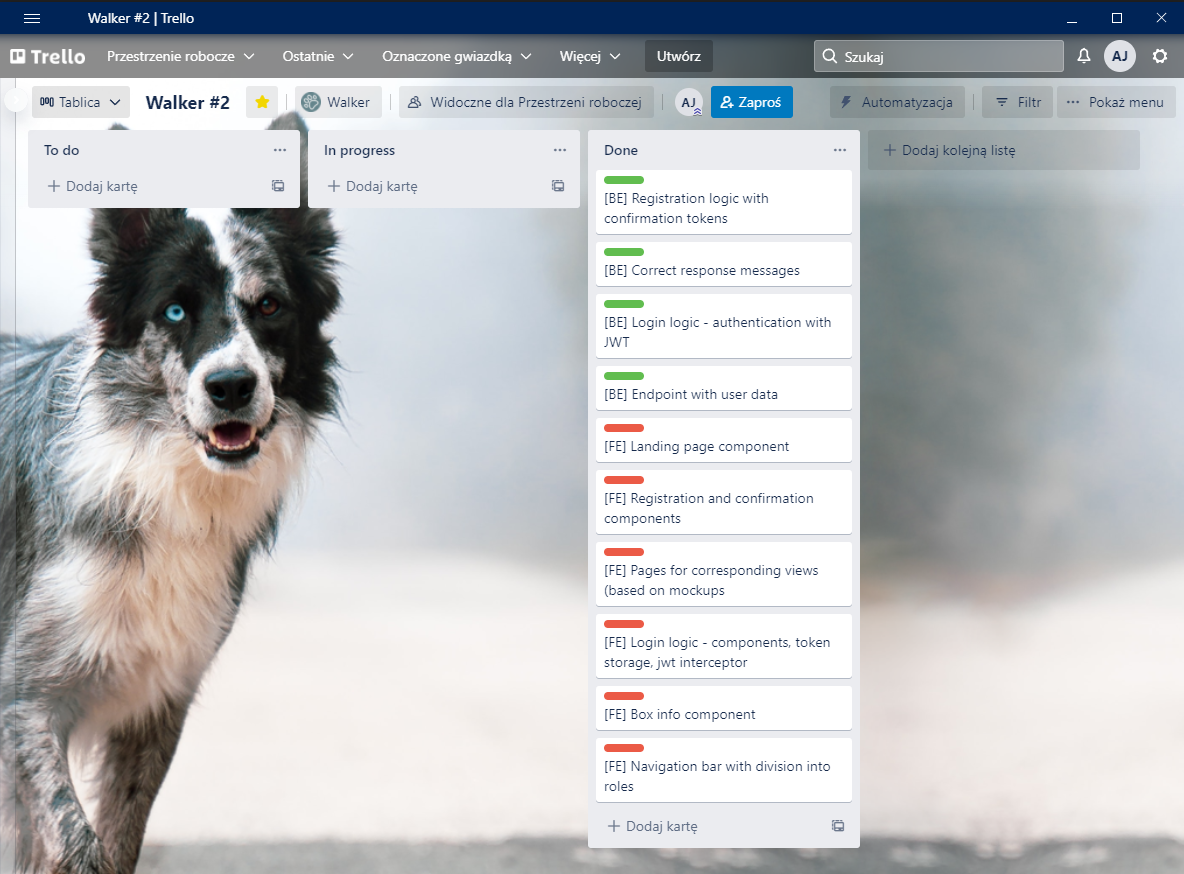
\includegraphics[width=0.7\linewidth]{rysunki/w2.PNG}
    \caption{Trello - tablica do drugiego etapu}
    \label{fig:walker-board-2}
\end{figure}  

\section{Adobe XD -- projektownaie prototypów}
Paleta kolorów taka i taka, z tego i tamtego zdjęcia

\begin{figure}[H]
    \centering
      \begin{tabular}{@{}ll@{}}
        
\includegraphics[width=0.475\textwidth]{rysunki/Start.png} & 
        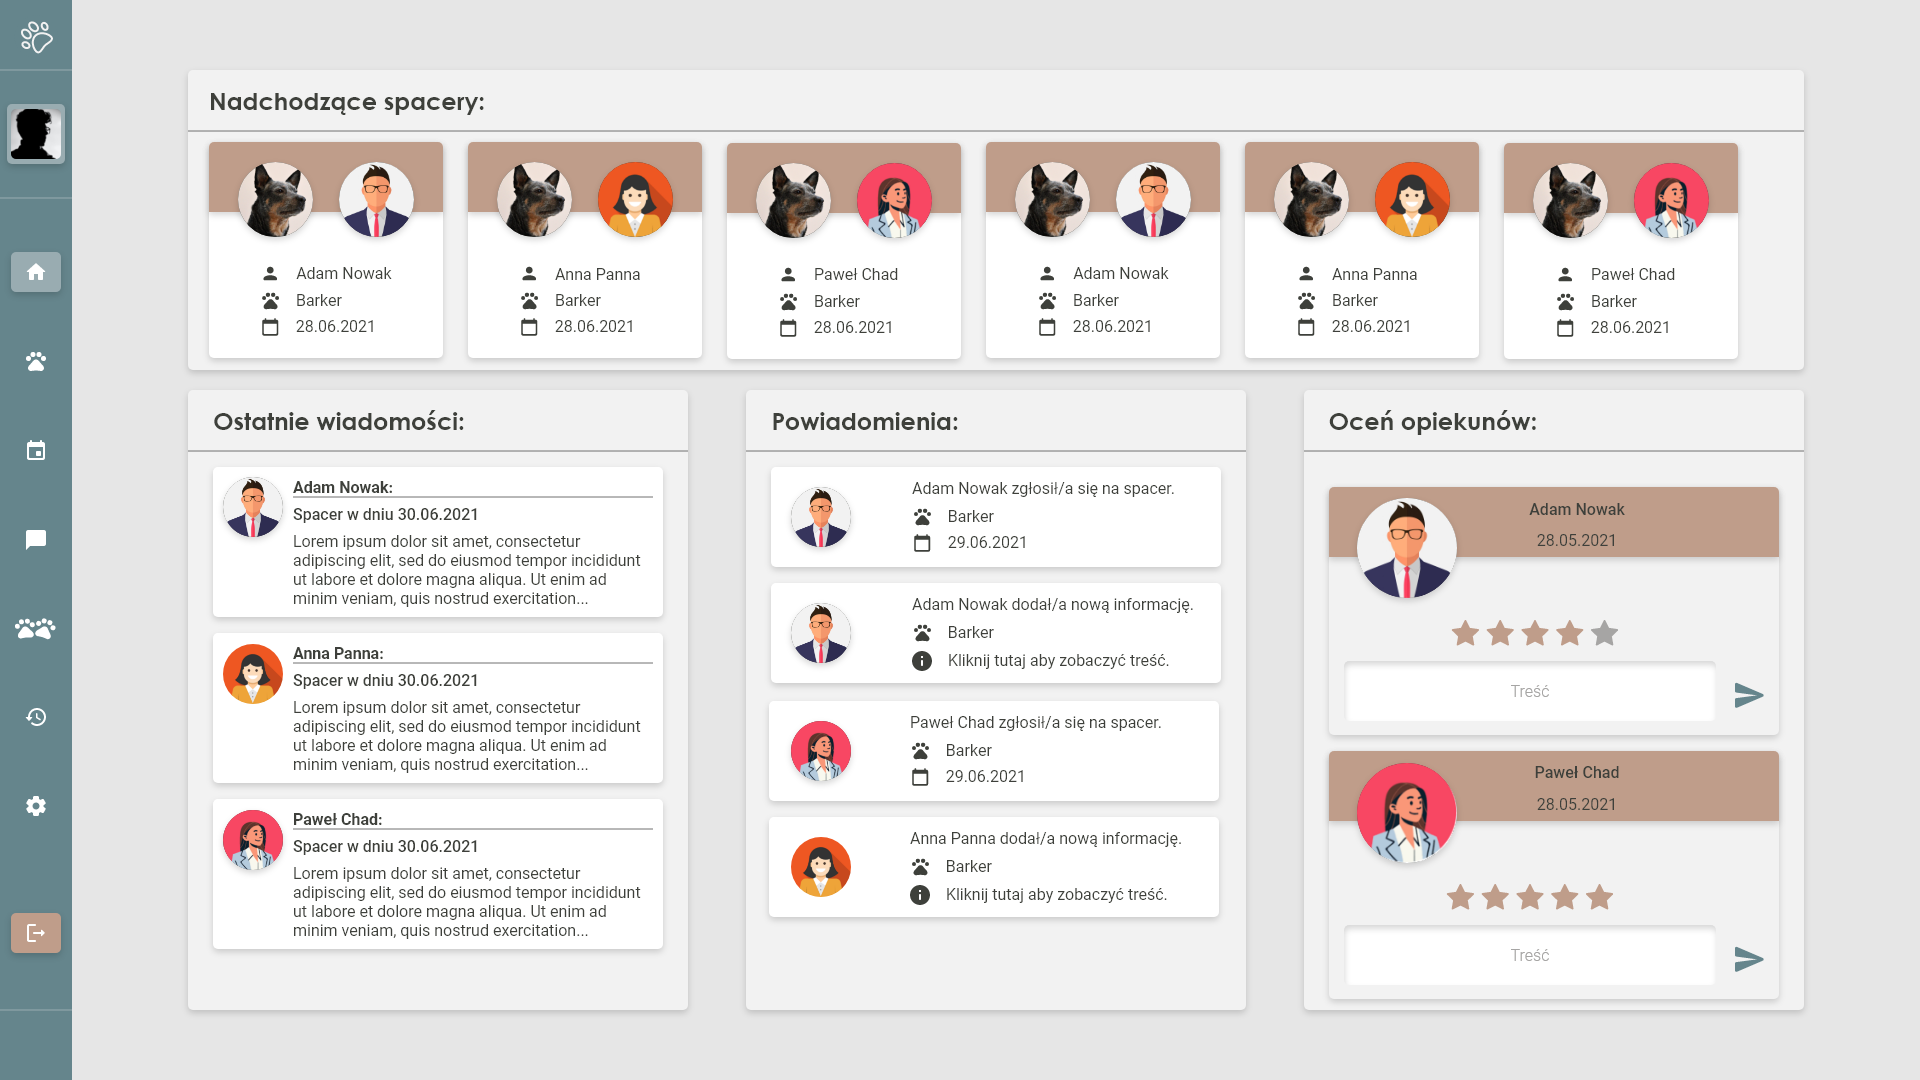
\includegraphics[width=0.475\textwidth]{rysunki/Home - owner.png}
      \end{tabular}
    \caption{Przykładowe prototypy aplikacji -- widok startowy, widok dashboardu}
    \label{fig:mocks-start-dashboard}
\end{figure}

\begin{figure}[H]
    \centering
      \begin{tabular}{@{}ll@{}}
        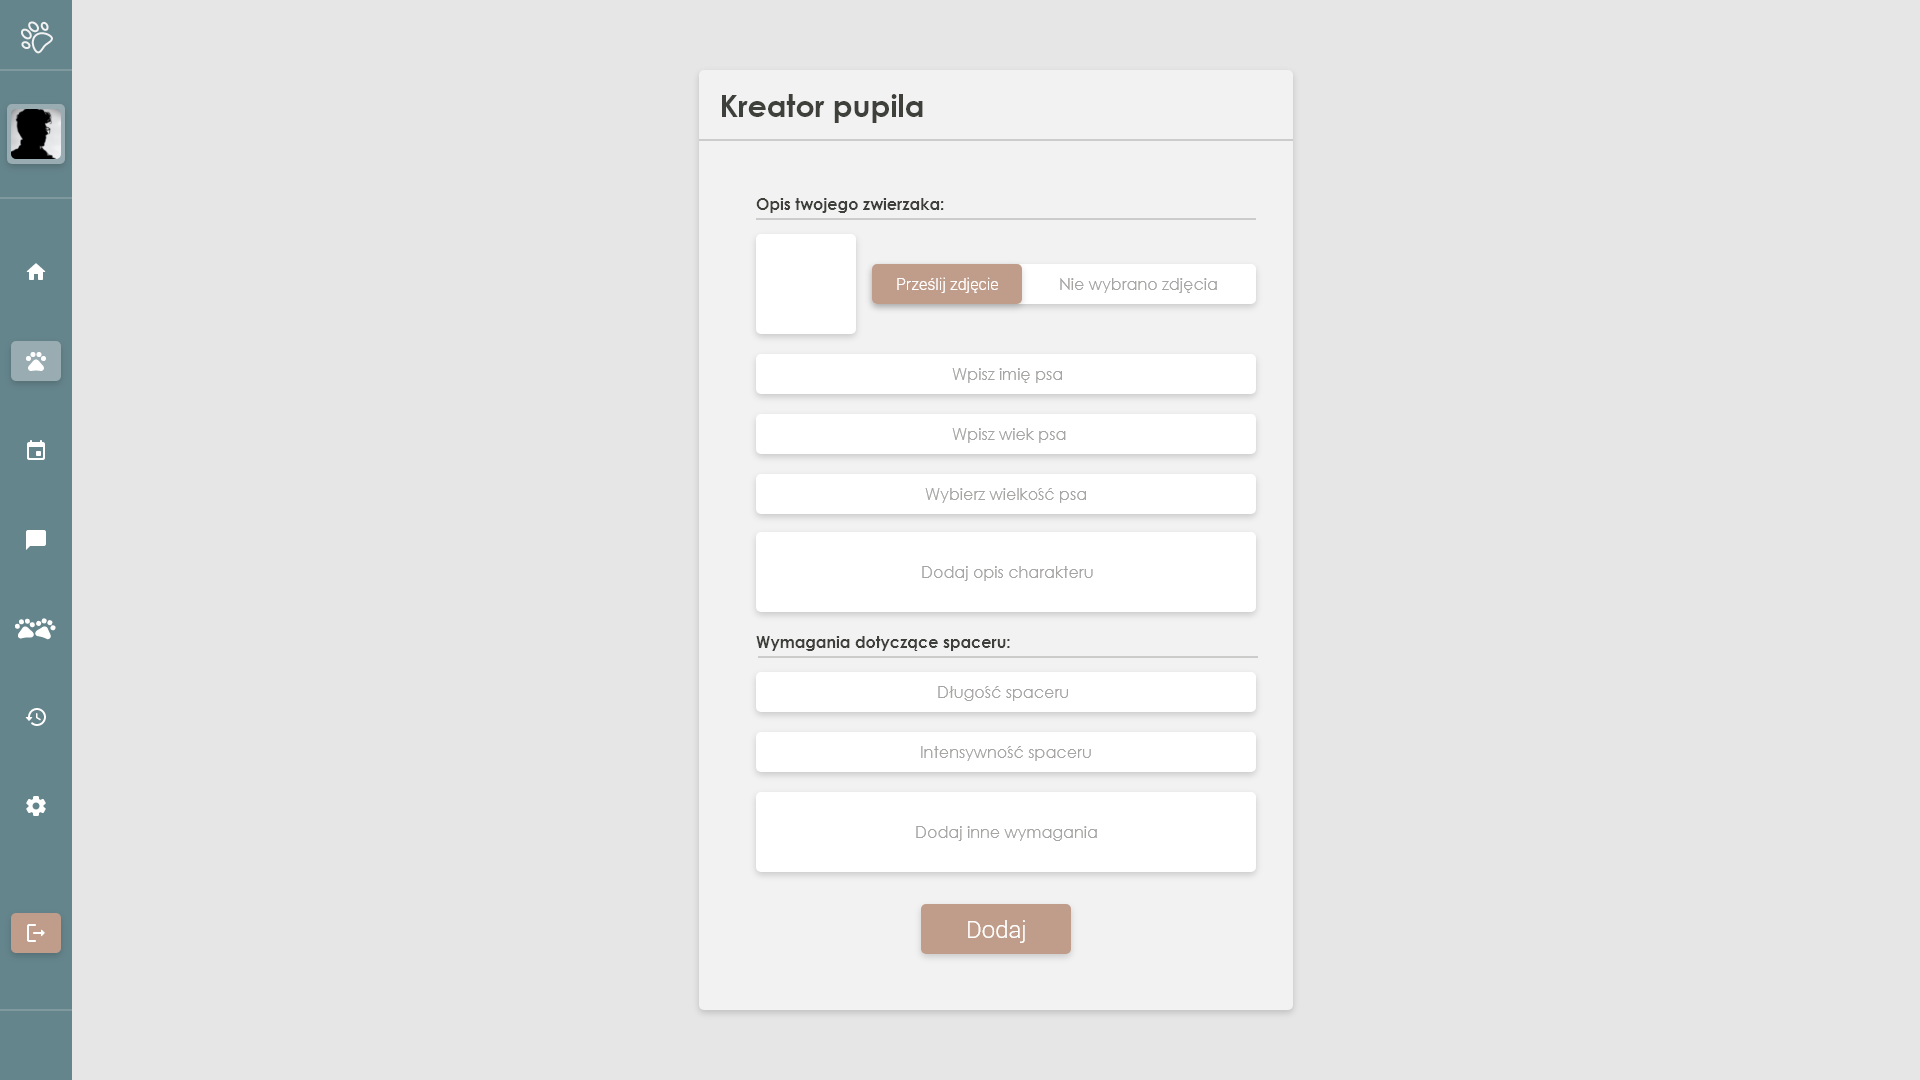
\includegraphics[width=0.475\textwidth]{rysunki/Home - dog creator.png} & 
        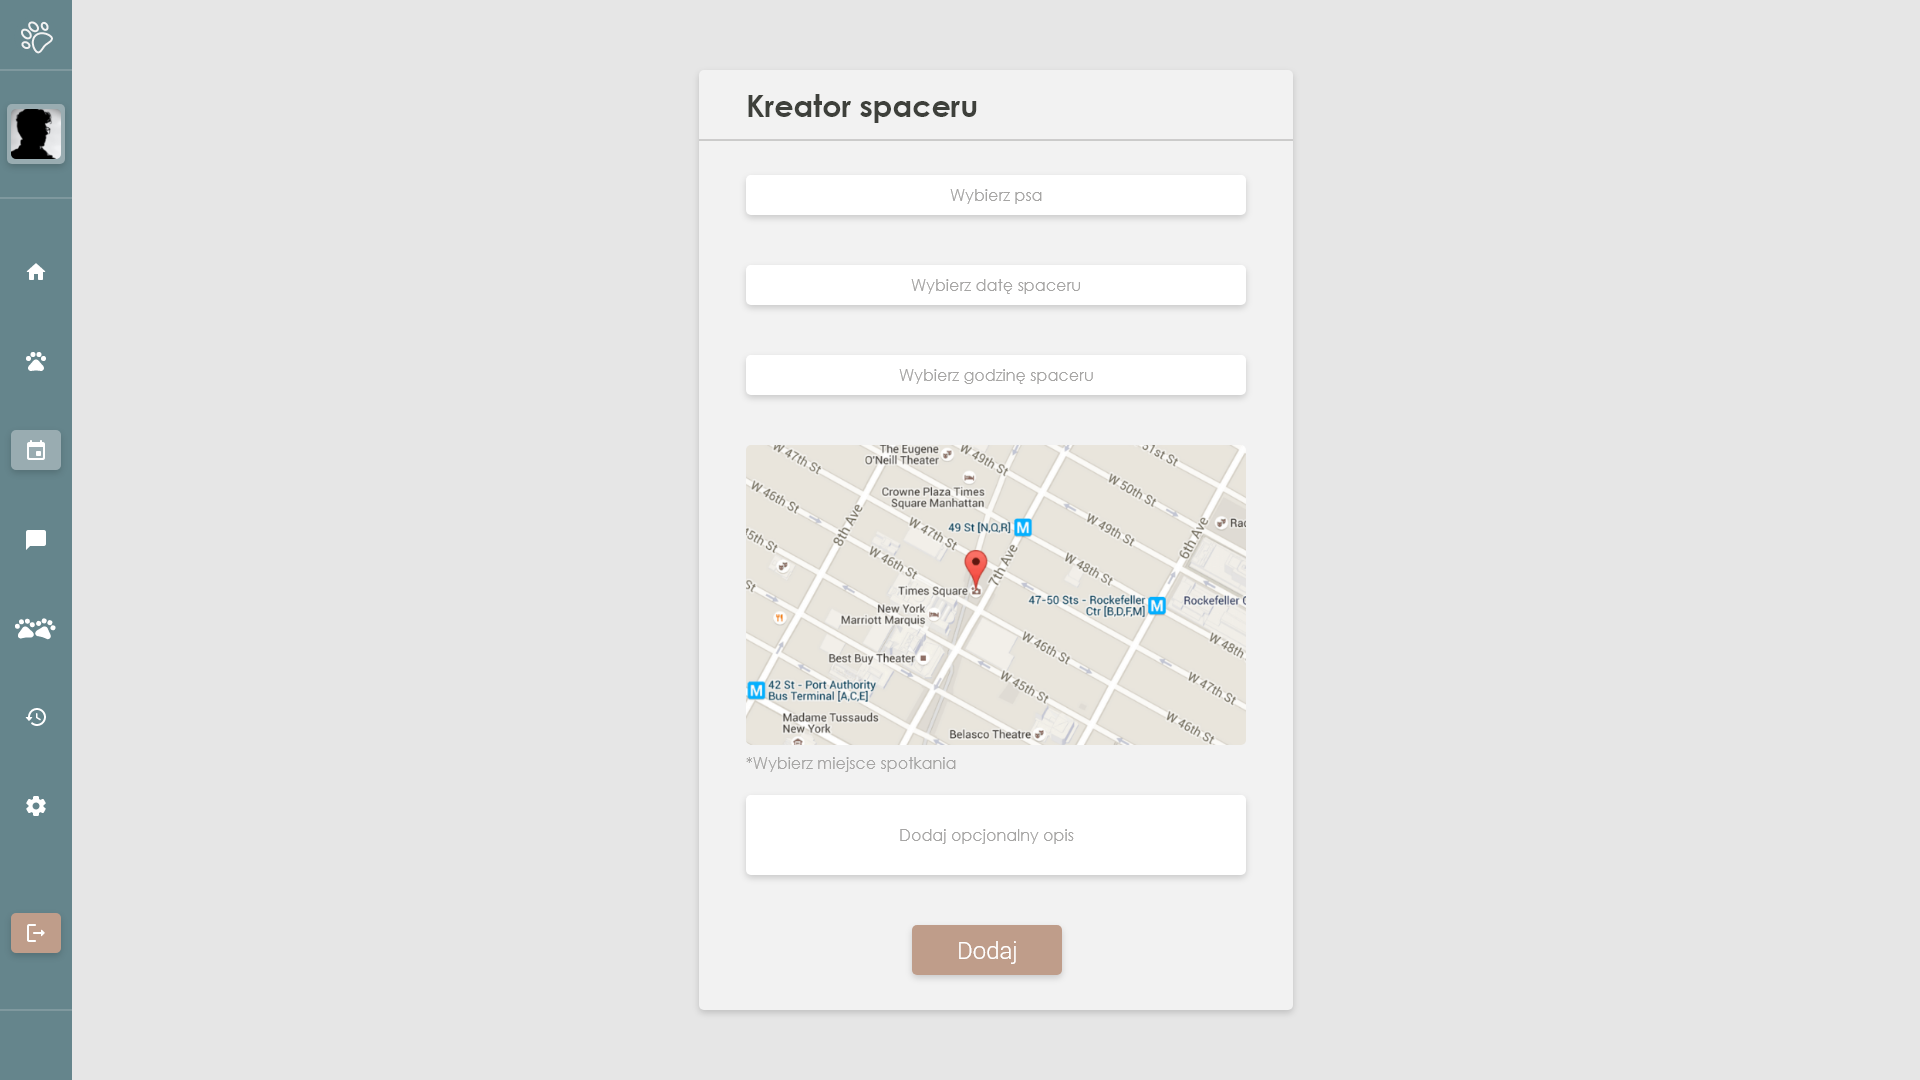
\includegraphics[width=0.475\textwidth]{rysunki/Home - walk creator.png}
      \end{tabular}
    \caption{Przykładowe prototypy aplikacji -- widok startowy, widok dashboardu}
    \label{fig:mocks-creators}
\end{figure}

\begin{figure}[H]
    \centering
      \begin{tabular}{@{}ll@{}}
        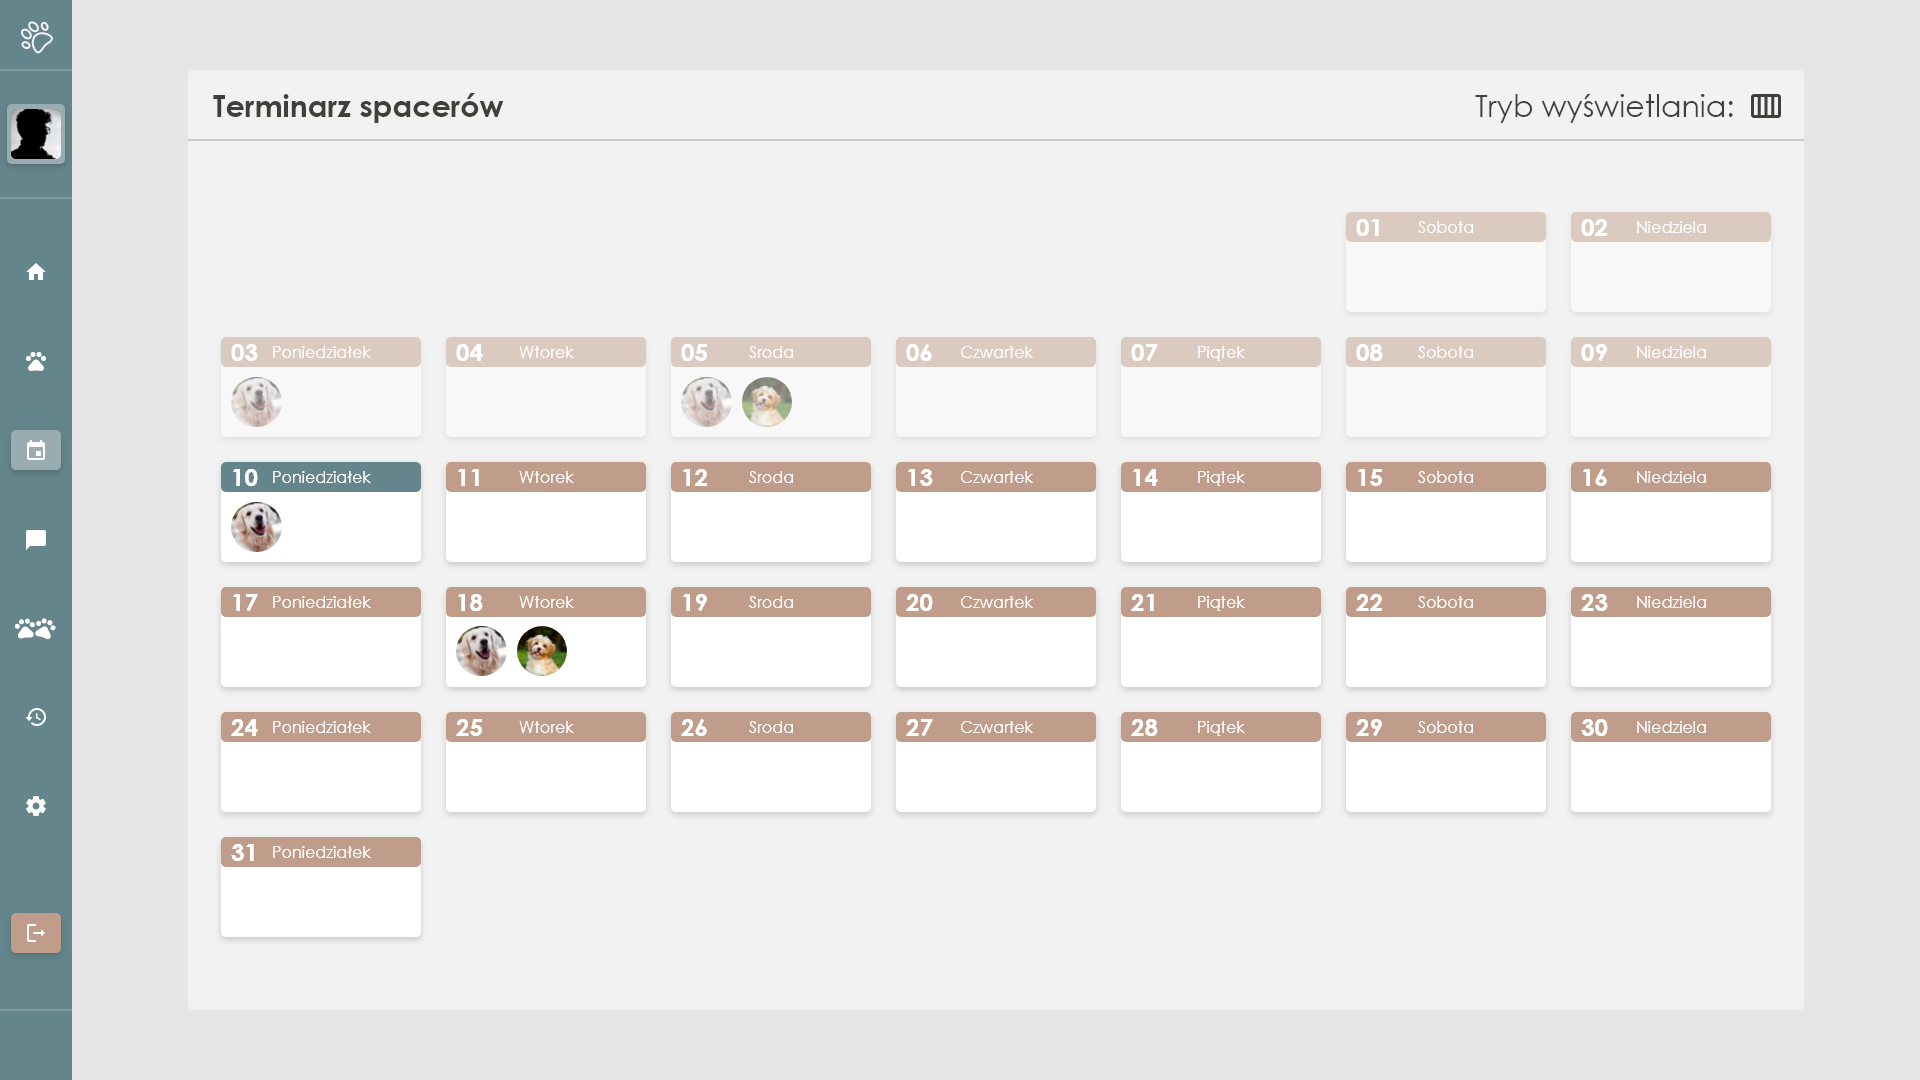
\includegraphics[width=0.475\textwidth]{rysunki/Home - walk calendar month.png} & 
        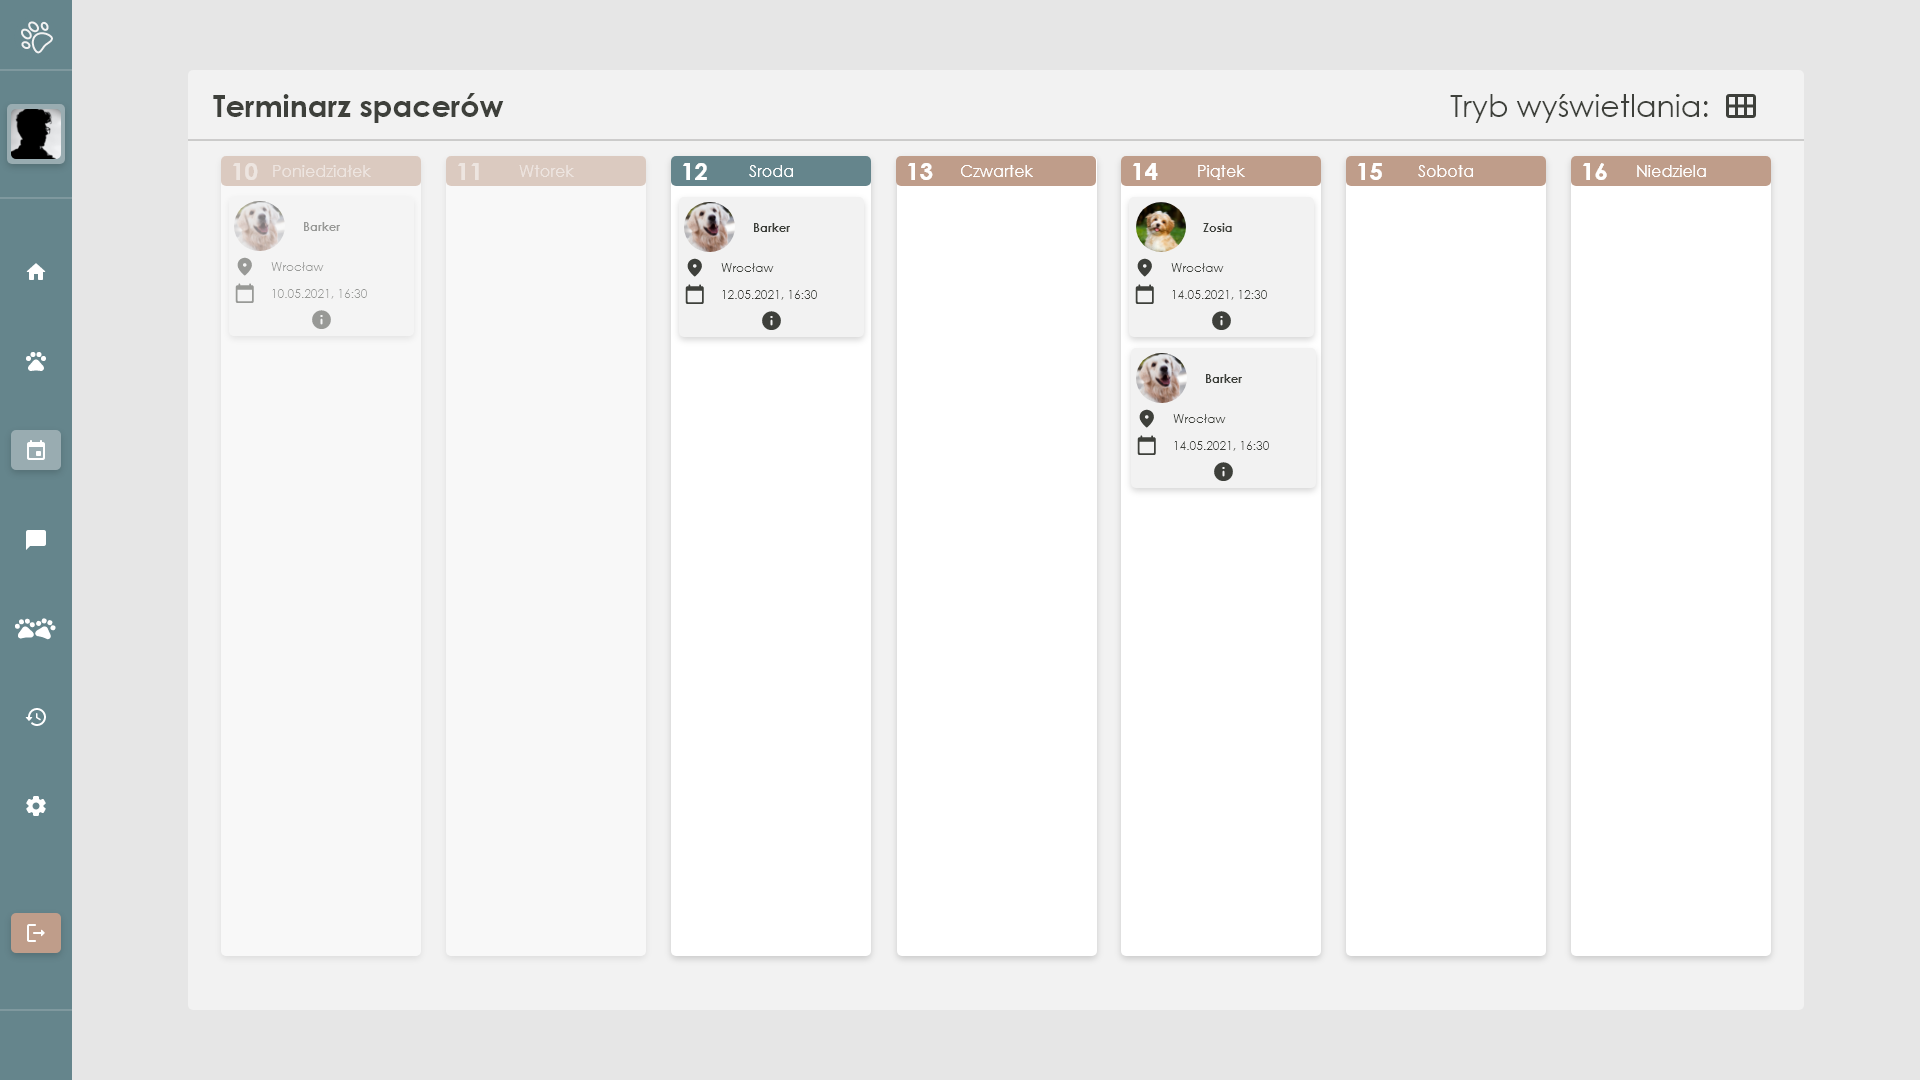
\includegraphics[width=0.475\textwidth]{rysunki/Home - walk calendar week.png}
      \end{tabular}
    \caption{Przykładowe prototypy aplikacji -- widok startowy, widok dashboardu}
    \label{fig:mocks-calendars}
\end{figure}

\begin{figure}[H]
    \centering
      \begin{tabular}{@{}ll@{}}
        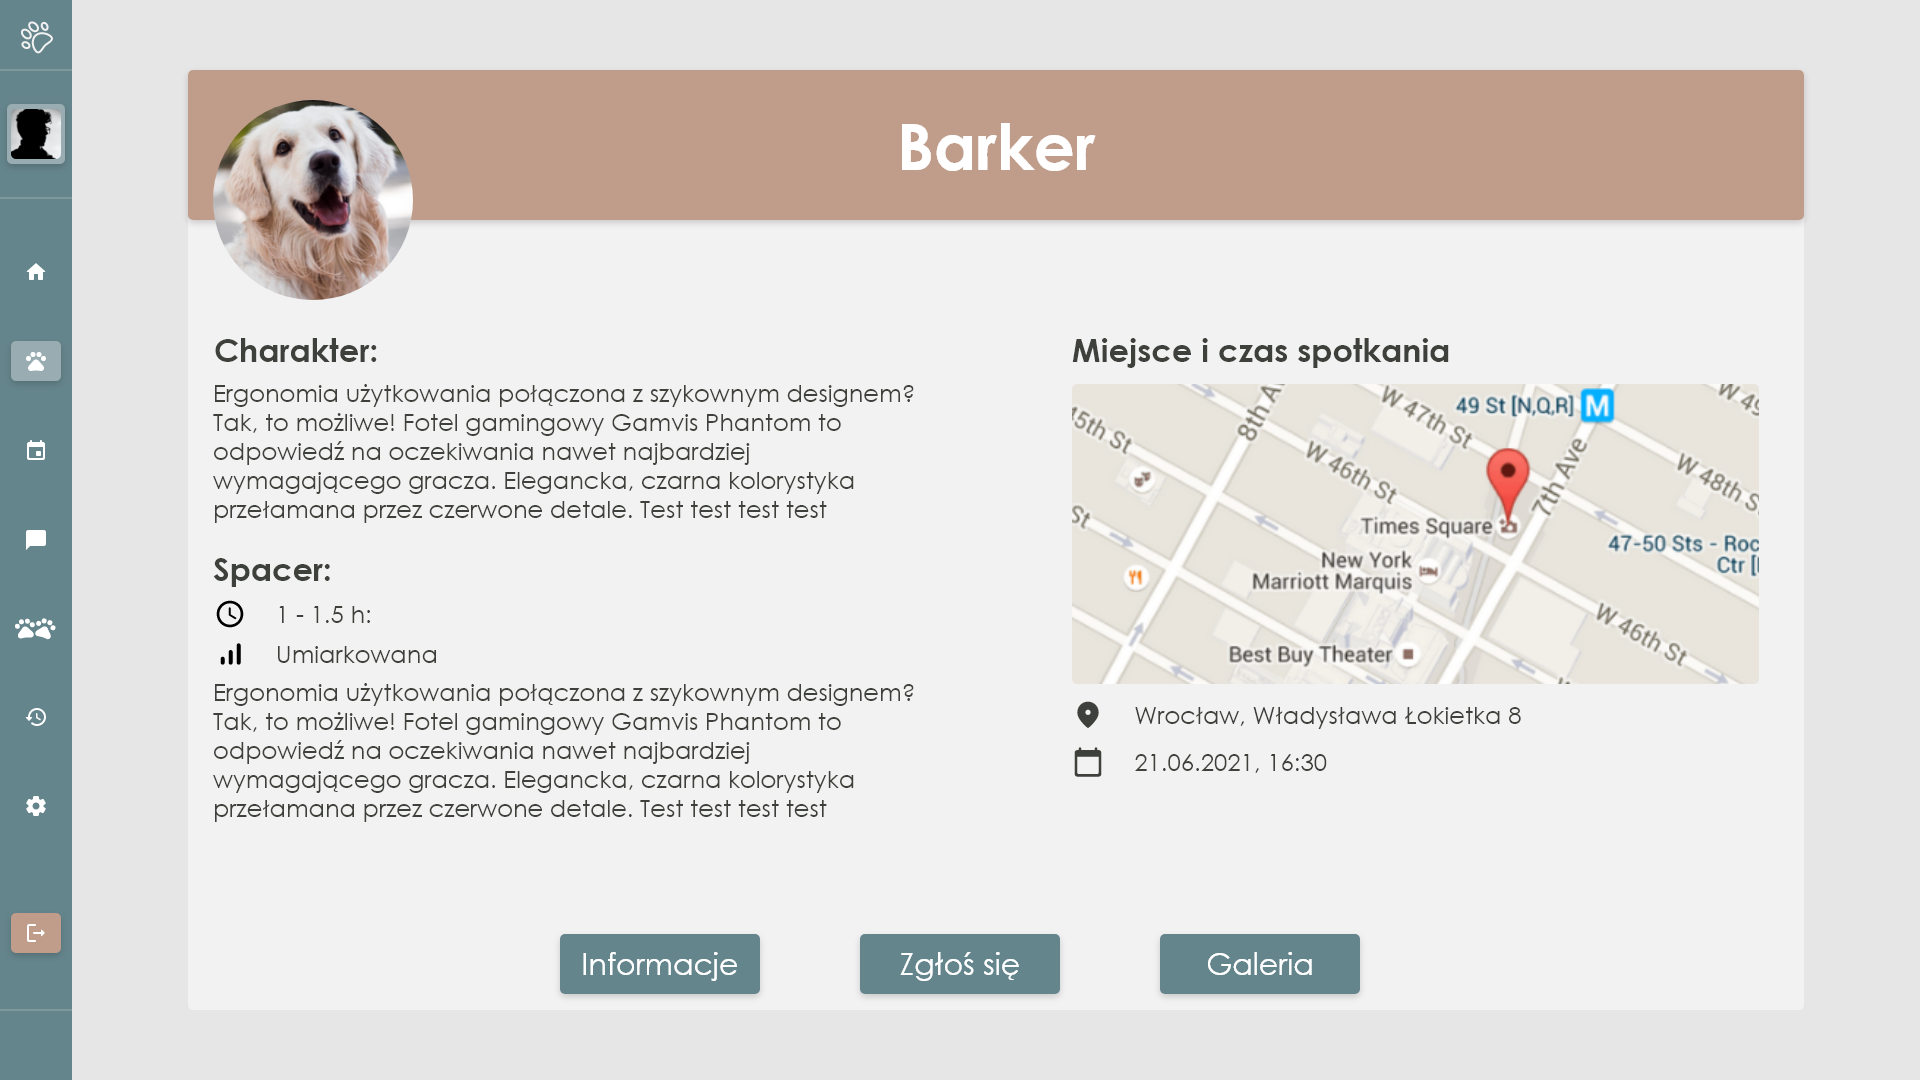
\includegraphics[width=0.475\textwidth]{rysunki/Home -walk info.png} & 
        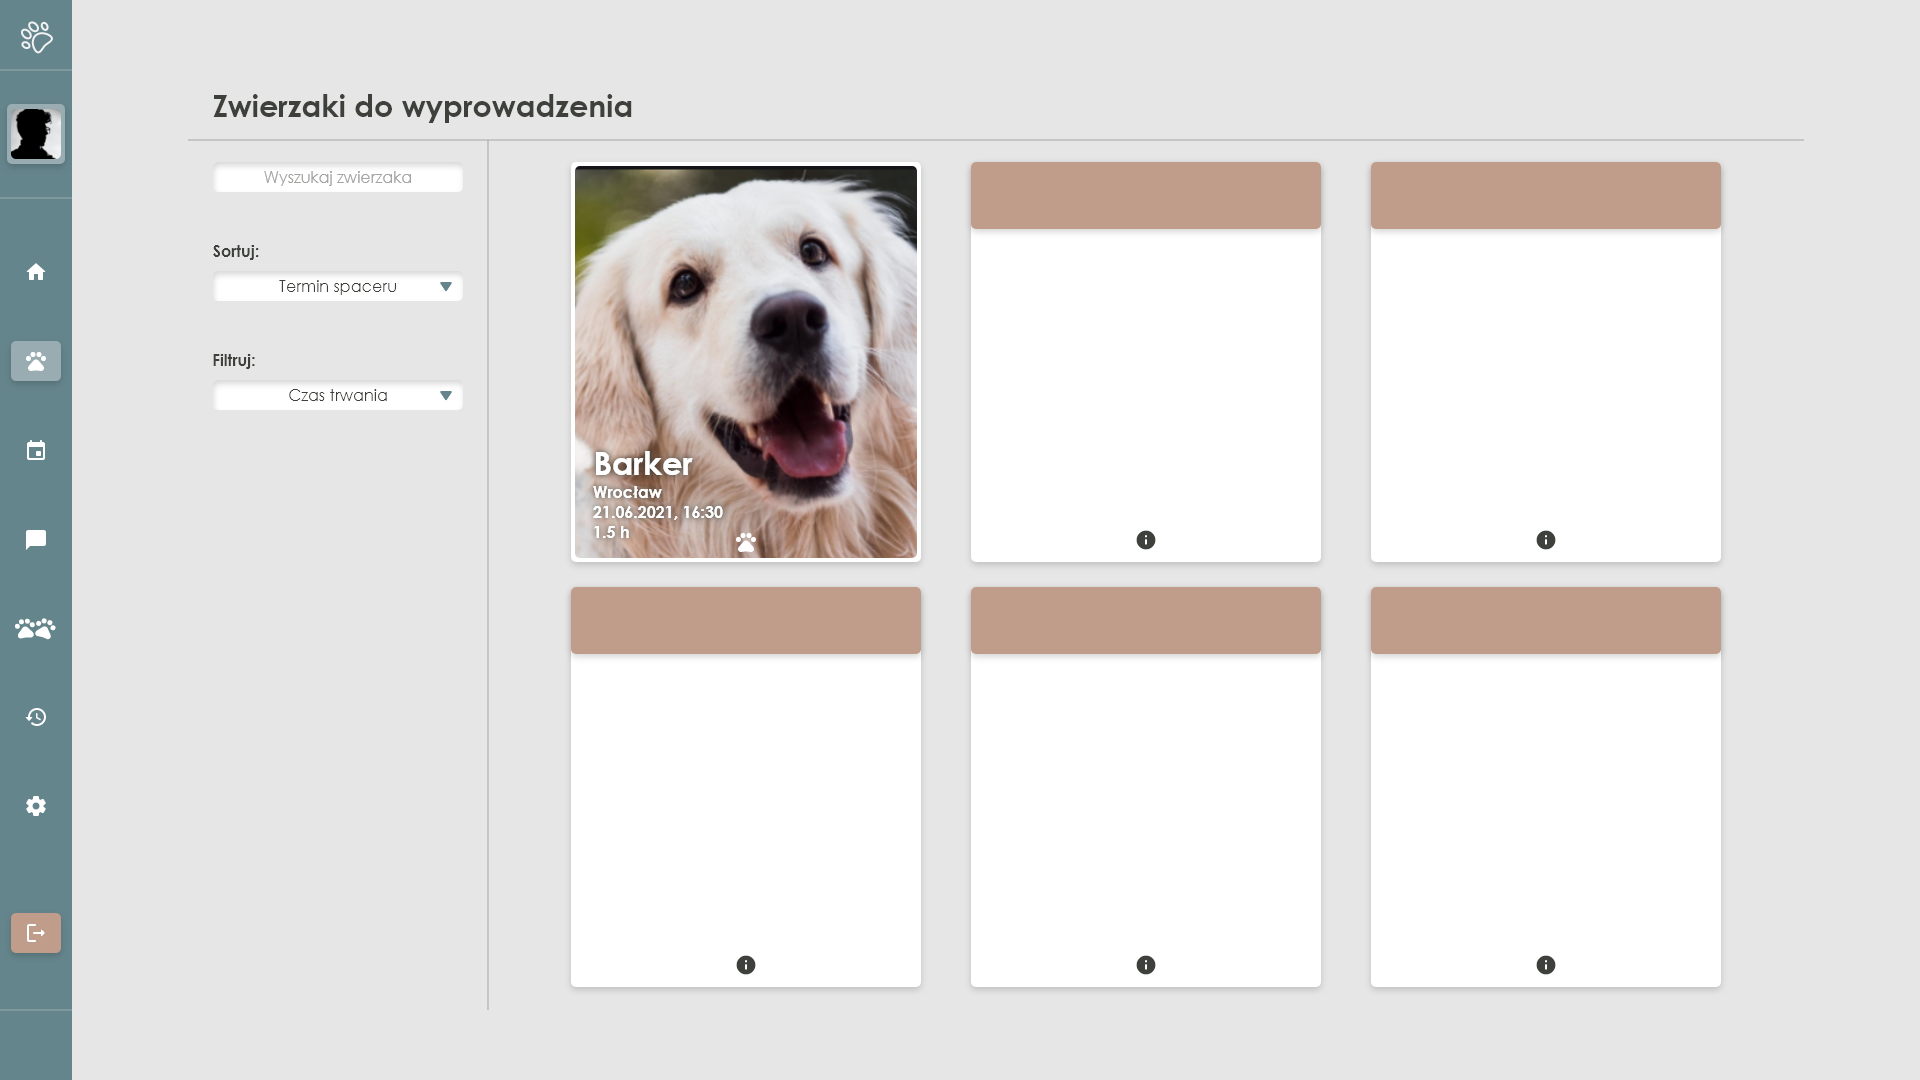
\includegraphics[width=0.475\textwidth]{rysunki/Home - dog list.png}
      \end{tabular}
    \caption{Przykładowe prototypy aplikacji -- widok startowy, widok dashboardu}
    \label{fig:mocks-lists}
\end{figure}

\newpage
\section{Java -- serce aplikacji}
\begin{figure}[H]
  \centering
  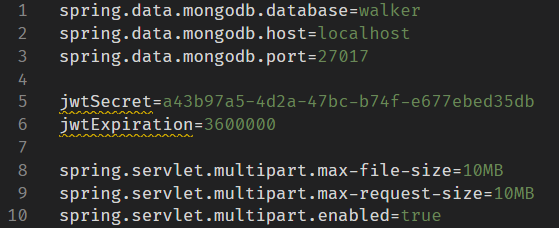
\includegraphics[width=1\linewidth]{rysunki/props.PNG}
  \caption{XYZ}
  \label{fig:xyz}
\end{figure}

\subsection{Architektura projektu}
Do zachowania porządku w projekcie zdecydowano się na zastosowanie odpowiedniej architektury projektu.

\begin{figure}[H]
  \centering
  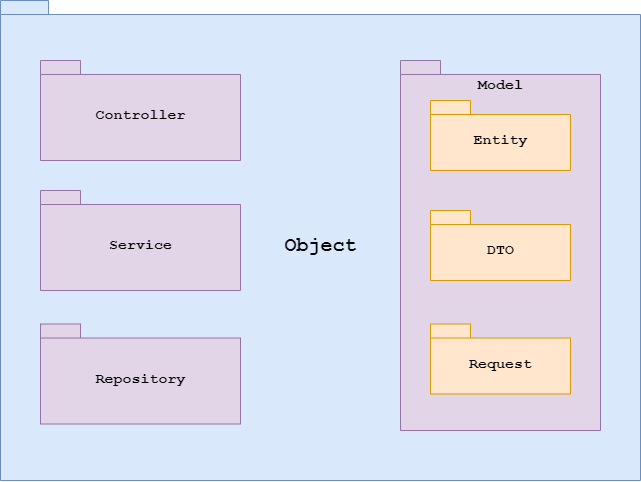
\includegraphics[width=0.7\linewidth]{rysunki/packages.png}
  \caption{Architektura projetku backendowego}
  \label{fig:java-architecture-2}
\end{figure}

Postanowiono na podzielenie głównych folderów ze względu na konkretne obiekty.
W folderach głównych znajdują się podfoldery odpowiedzialne za przechowywanie: 
\begin{itemize}[leftmargin=1cm]
  \item \textit{Controller} -- przechowuje plik kontrolera, który udostępnia endpointy;
  \item \textit{Service} -- przechowuje plik serwisu, który posiada główną logikę związaną z danym obiektem;
  \item \textit{Repository} -- przechowuje plik repozytorium obiektu potrzebnego do komunikacji z bazą danych;
  \item \textit{Model}:
  \begin{itemize}
    \item \textit{Entity} -- obiekt rzutowany bezpośrednio na bazę danych;
    \item \textit{DTO} -- obiekt wysyłany do aplikacji dostępowej, bardziej rozbudowana encja o dodatkowe pola;
    \item \textit{Request} -- obiekt przesyłany bezpośrednio z aplikacji dostepowej po wypełnieniu formularzu;
  \end{itemize}
\end{itemize}

\begin{figure}[H]
  \centering
  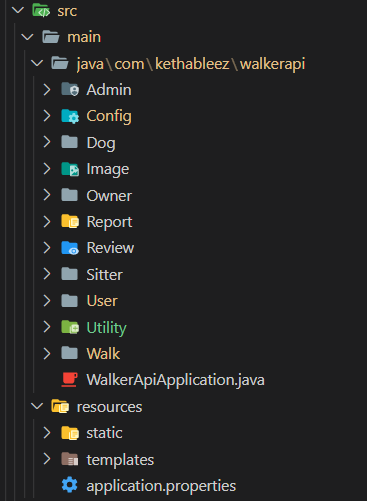
\includegraphics[width=0.5\linewidth]{rysunki/arch-java.PNG}
  \caption{Architektura projetku backendowego}
  \label{fig:java-architecture}
\end{figure}

\subsection{Zbiór endpointów}
\begin{figure}[H]
    \centering
    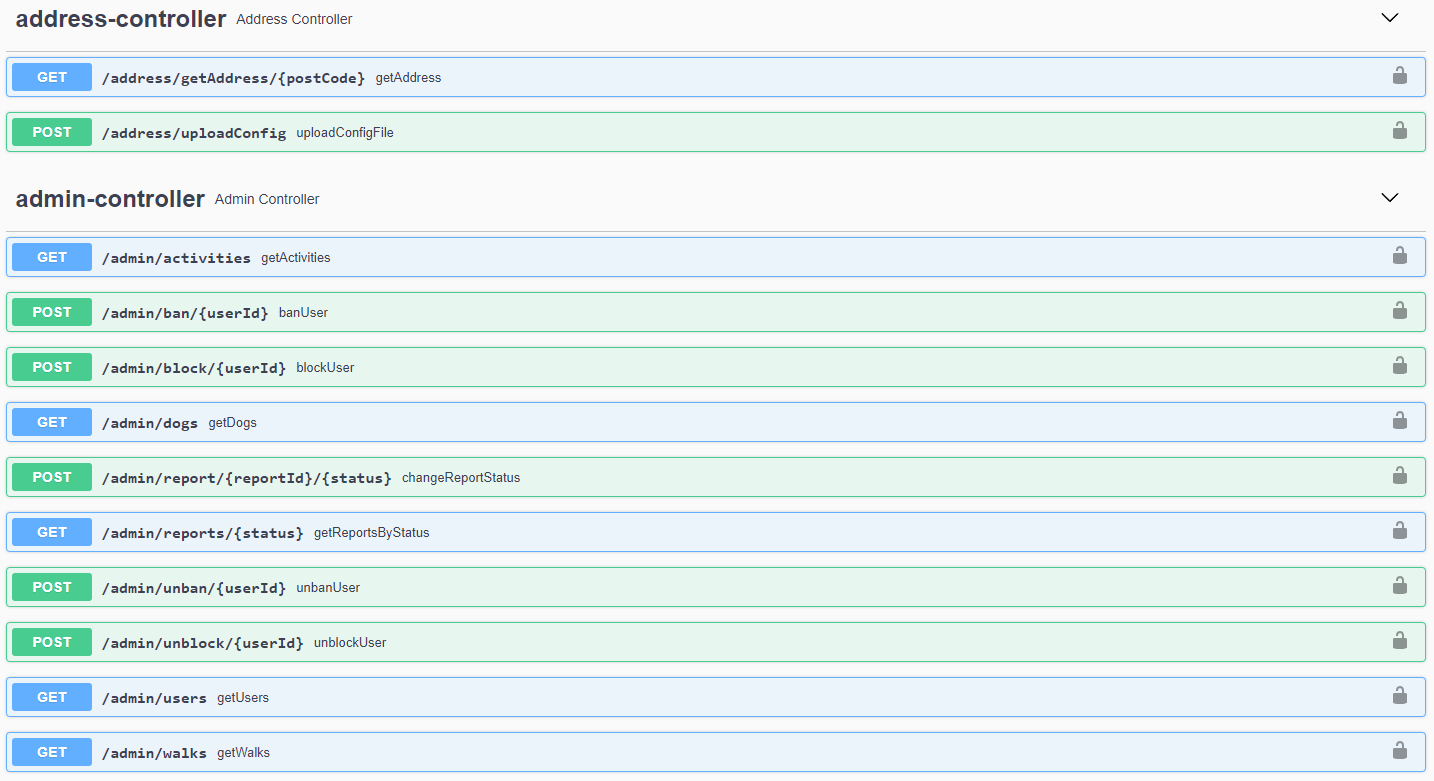
\includegraphics[width=0.7\linewidth]{rysunki/sw-1.PNG}
    \caption{Dokumentacja 1}
    \label{fig:swagger-1}
\end{figure}  
\begin{figure}[H]
    \centering
    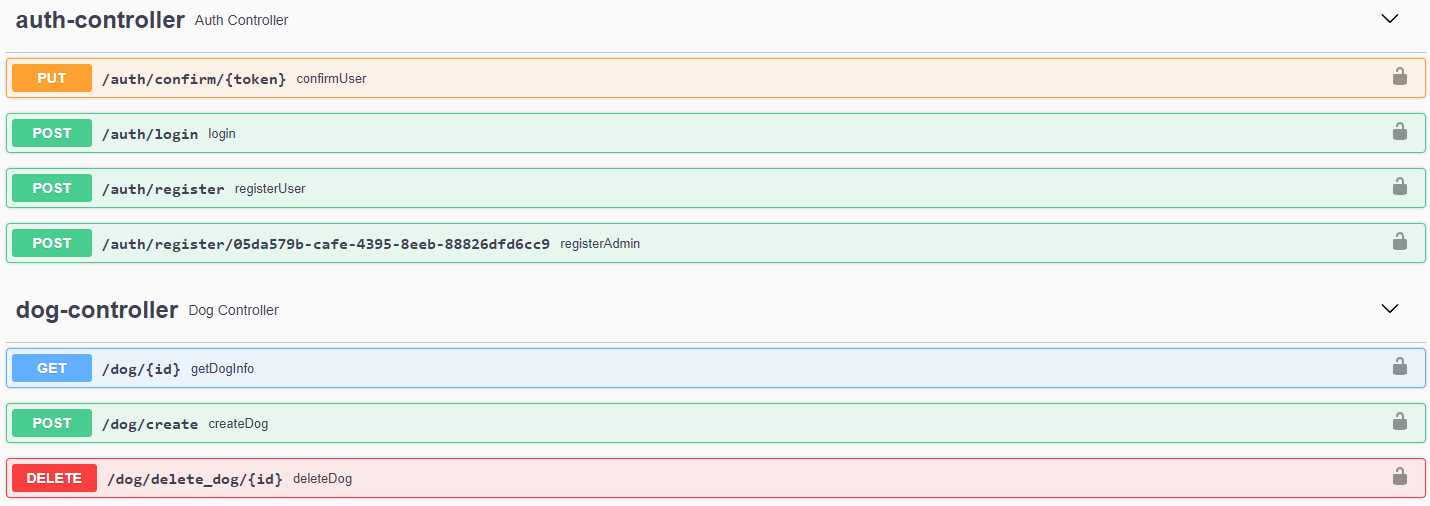
\includegraphics[width=0.7\linewidth]{rysunki/sw-2.PNG}
    \caption{Dokumentacja 2}
    \label{fig:swagger-2}
\end{figure}  
\begin{figure}[H]
    \centering
    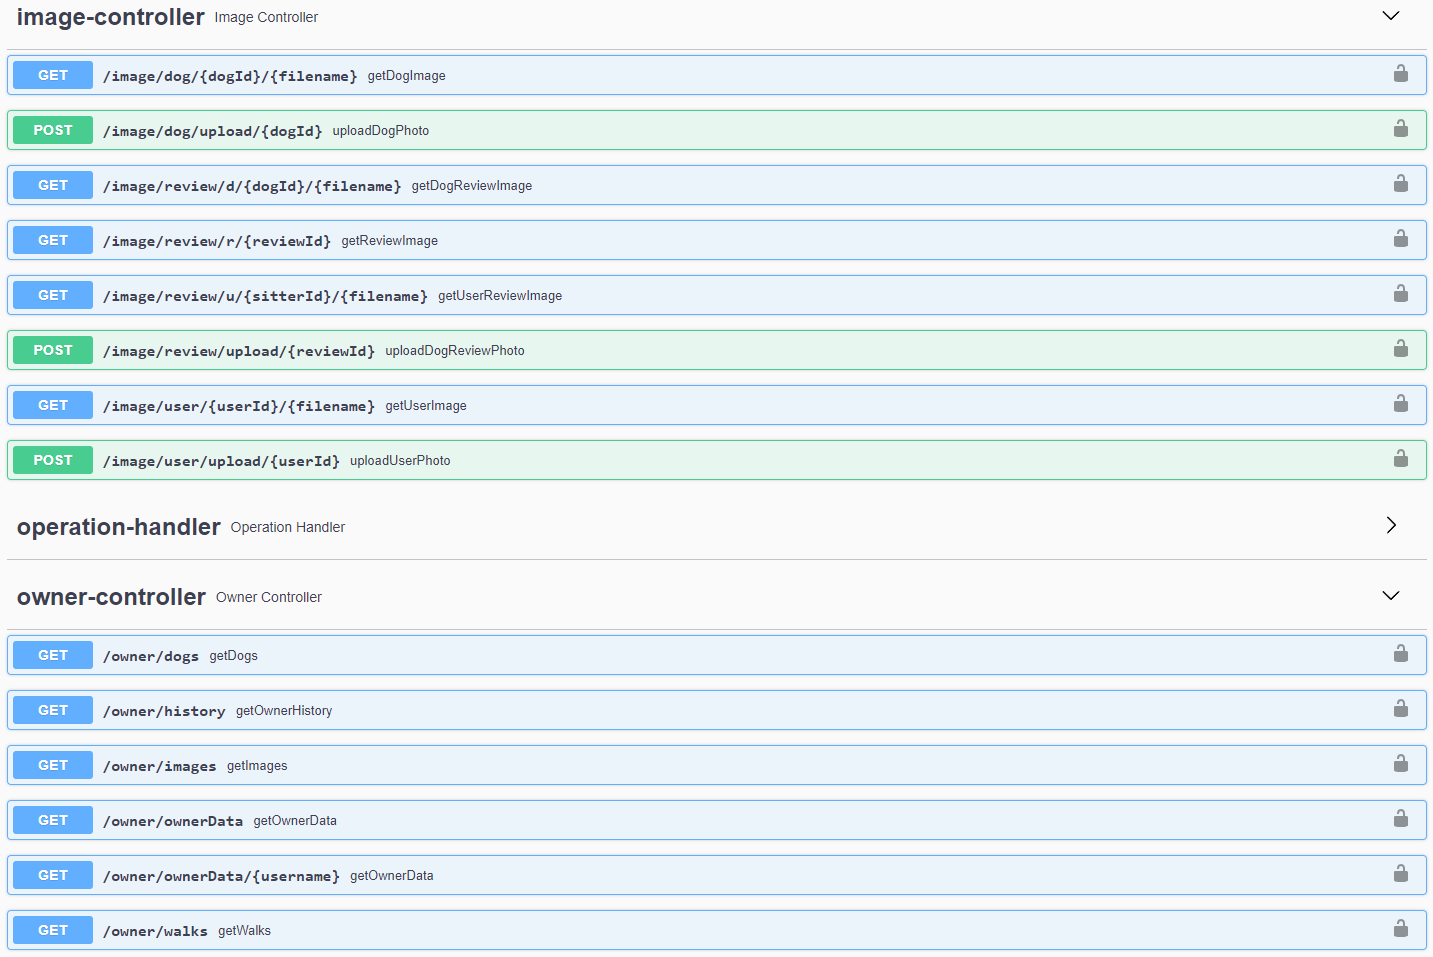
\includegraphics[width=0.7\linewidth]{rysunki/sw-3.PNG}
    \caption{Dokumentacja 3}
    \label{fig:swagger-3}
\end{figure}  
\begin{figure}[H]
    \centering
    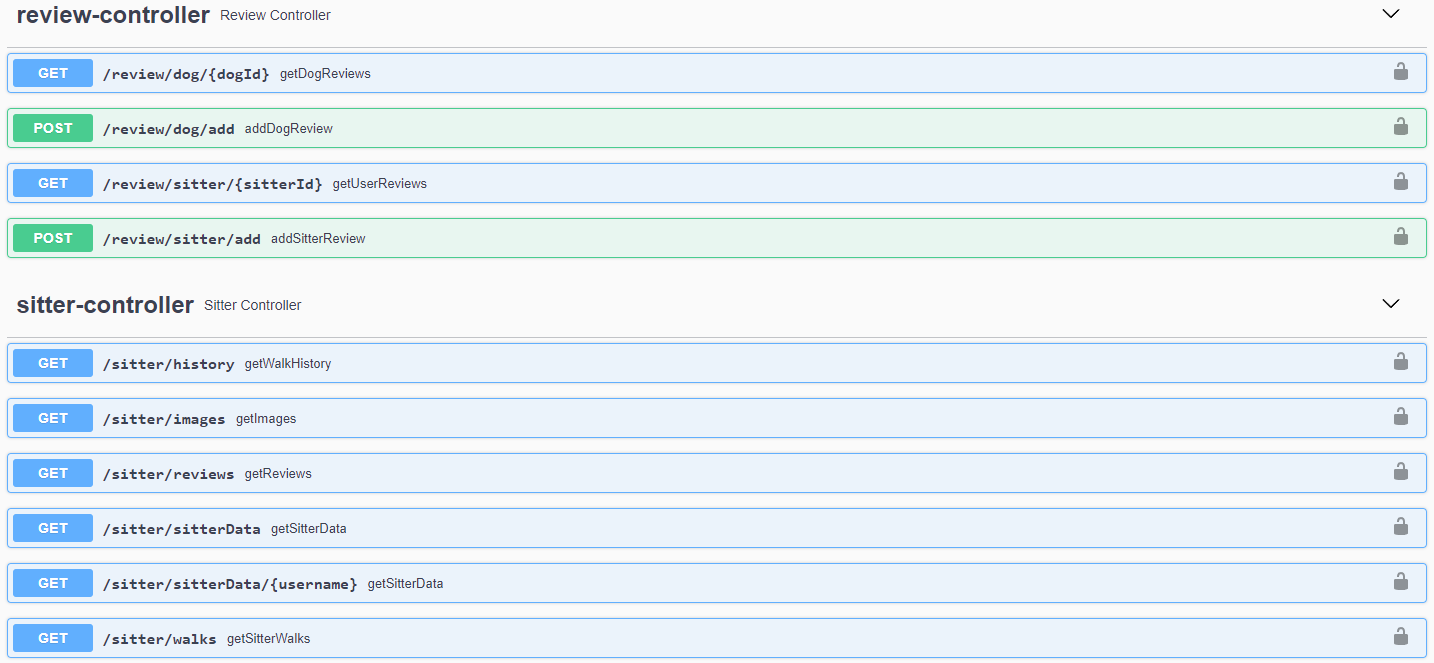
\includegraphics[width=0.7\linewidth]{rysunki/sw-4.PNG}
    \caption{Dokumentacja 4}
    \label{fig:swagger-4}
\end{figure}  
\begin{figure}[H]
    \centering
    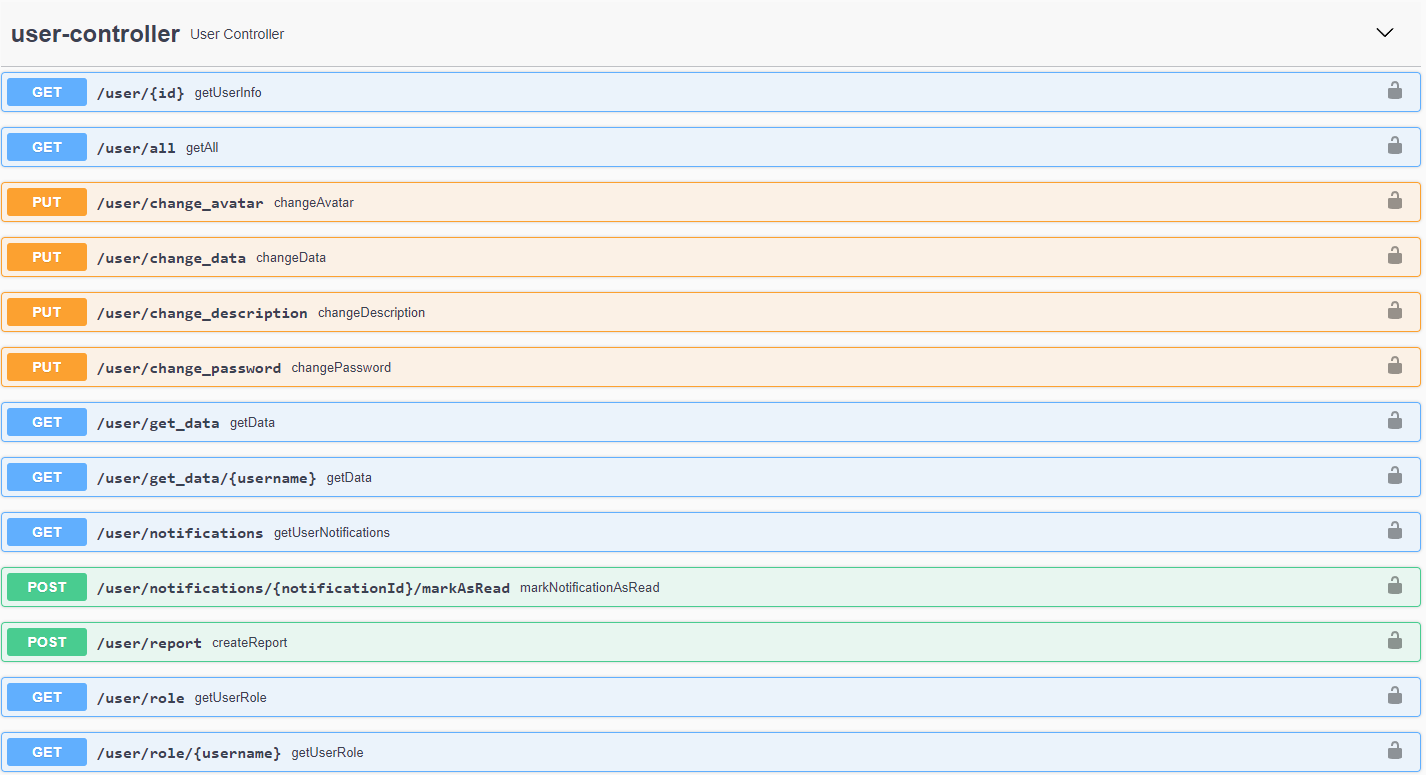
\includegraphics[width=0.7\linewidth]{rysunki/sw-5.PNG}
    \caption{Dokumentacja 5}
    \label{fig:swagger-5}
\end{figure}  
\begin{figure}[H]
    \centering
    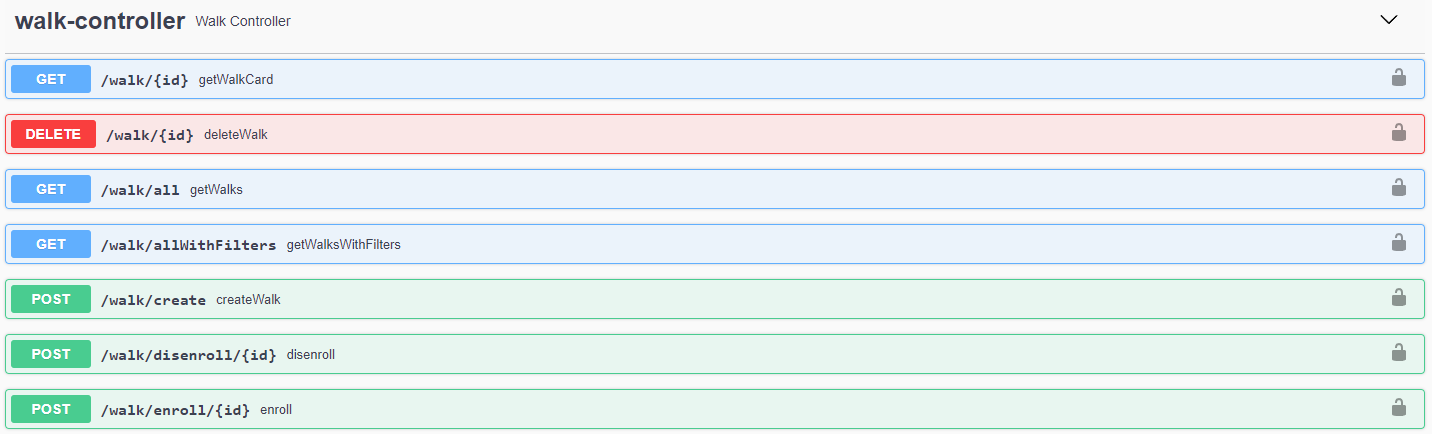
\includegraphics[width=0.7\linewidth]{rysunki/sw-6.PNG}
    \caption{Dokumentacja 6}
    \label{fig:swagger-6}
\end{figure}  
\subsection{JWT -- Autoryzacja i autentykacja}
\begin{figure}[H]
  \centering
  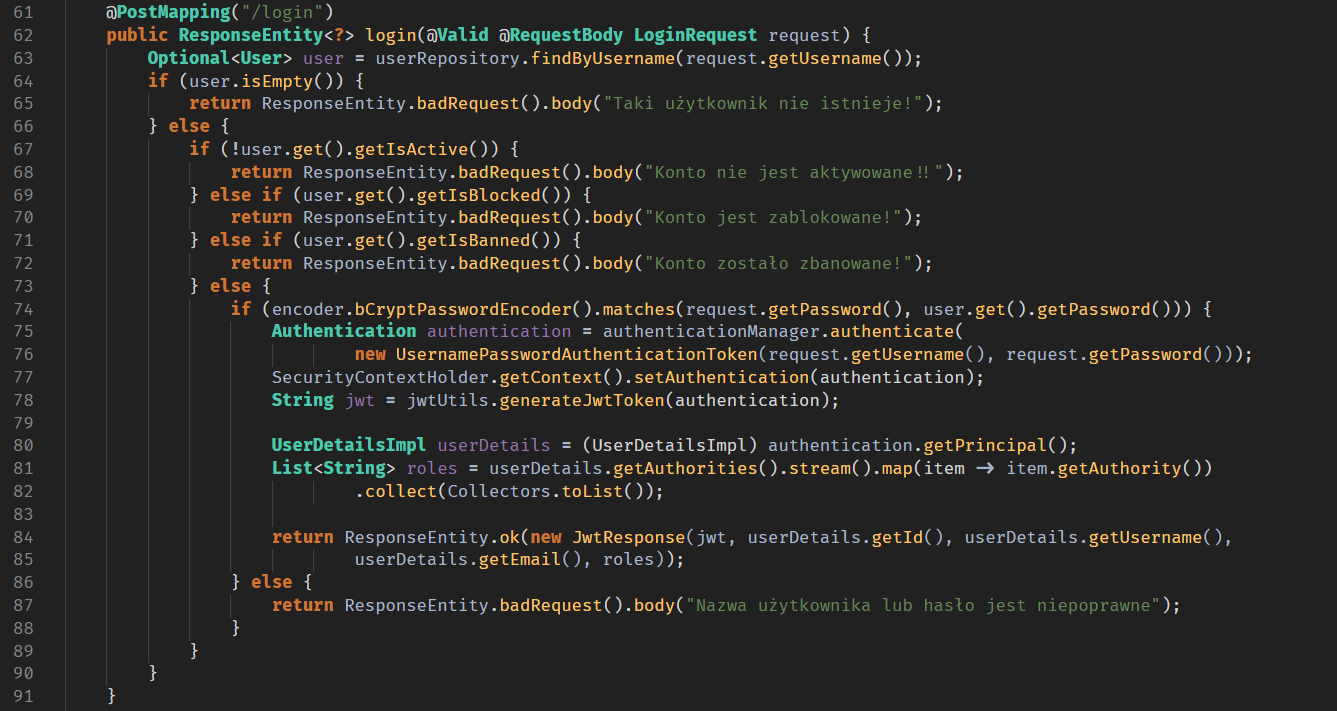
\includegraphics[width=1\linewidth]{rysunki/login.PNG}
  \caption{Implementacja logowania przy pomocy JWT}
  \label{fig:JWT}
\end{figure}  

\subsection{Implementacja wyszukiwania po lokalizacji}
w headerze przesyłany distCode a w backendzie filtrowana lista spacerów
\begin{figure}[H]
  \centering
  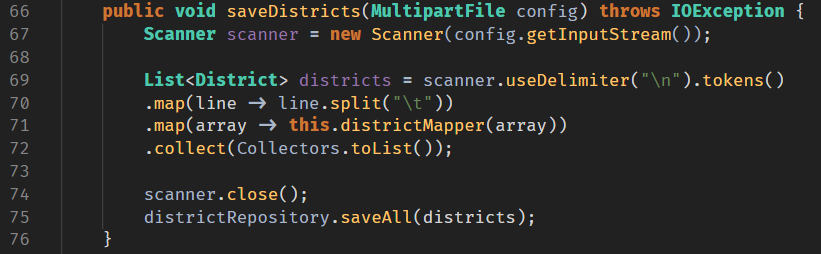
\includegraphics[width=1\linewidth]{rysunki/save.PNG}
  \caption{XYZ}
  \label{fig:xyz}
\end{figure}
\begin{figure}[H]
  \centering
  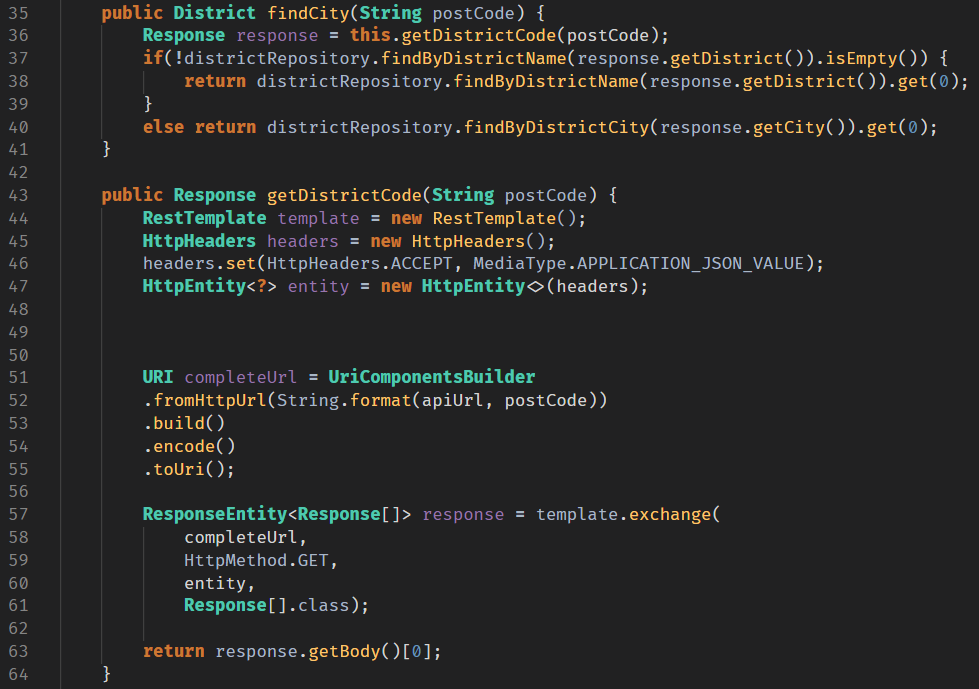
\includegraphics[width=1\linewidth]{rysunki/get-dist.PNG}
  \caption{XYZ}
  \label{fig:xyz}
\end{figure}

\subsection{Diagramy klas}

\subsection{Encje}
\begin{figure}[H]
  \centering
  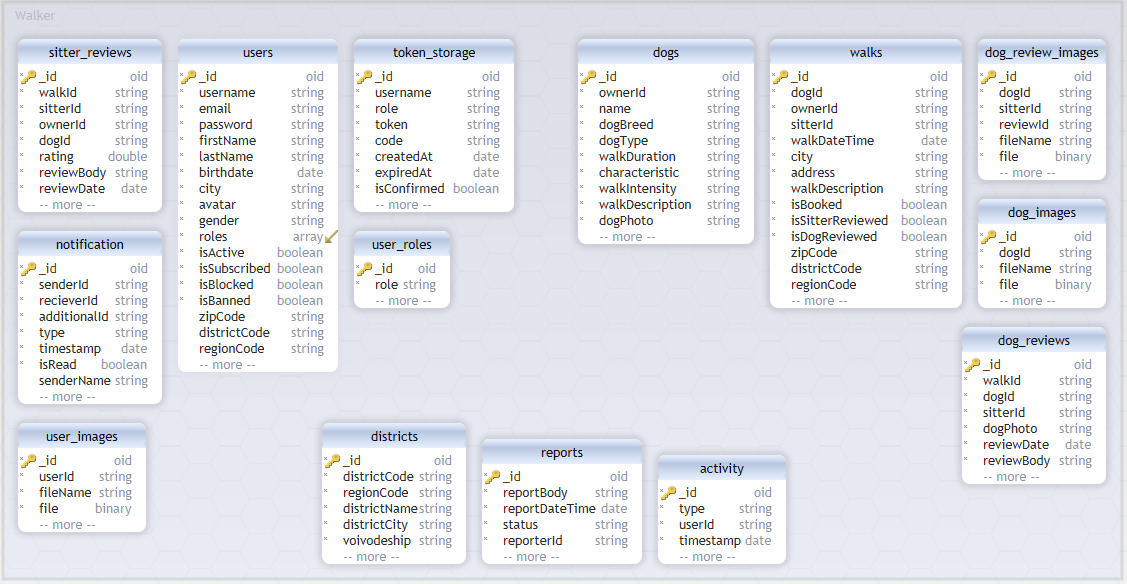
\includegraphics[width=1\linewidth]{rysunki/database.PNG}
  \caption{Widok bazy danych}
  \label{fig:database}
\end{figure}  

\newpage
\section{Angular -- warstwa dostępowa}
\subsection{Architektura projektu frontendowego}
\begin{figure}[H]
  \centering
  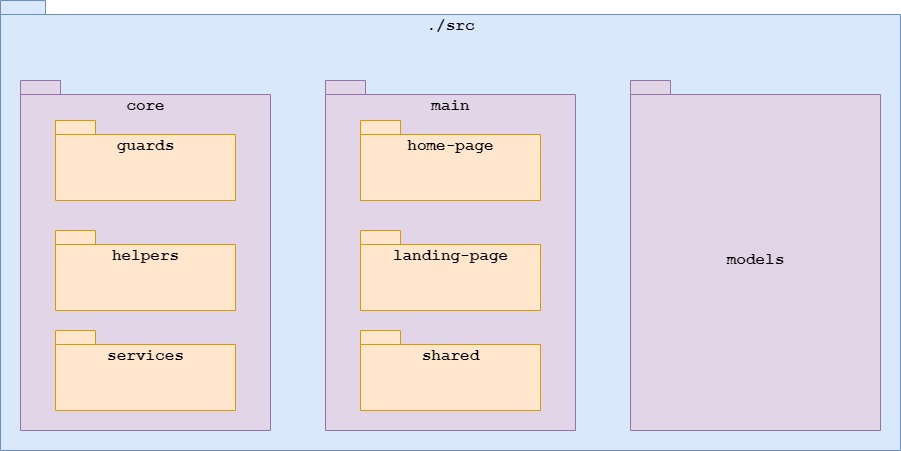
\includegraphics[width=1\linewidth]{rysunki/angular-arch.png}
  \caption{XYZ}
  \label{fig:xyz}
\end{figure}

\subsection{JWT -- Autoryzacja i autentykacja}

\subsection{Biblioteki i moduły}

\subsection{Konfiguracja projektu}